\documentclass[pflichtenheft.tex]{subfiles}

\begin{document}

\chapter{Graphische Benutzeroberfläche}
Auf den Endgeräten wird eine Graphische Benutzeroberfläche angezeigt. Diese soll sich je nach Endgerät nur im verfügbaren Platz entsprechend der Größe der Displays unterscheiden, nicht aber in der Funktionalität.

Der Nutzer soll GUI-Instrumente anzeigen und ausblenden können. Zu den GUI-Instrumenten gehören sowohl Dashes mit Echtzeitinformation, als auch Graphen, die Aufzeichnungen von Daten in einem längeren Zeitraum visualisieren.


\section{Dashboard}

Das Dashboard besteht aus verschiedenen Anzeigeelementen, sogenannten Dashes, und oben einer Leiste auf der verschiedene Informationen dargestellt werden. Links wird, beim Fahrer, ein Lenkrad angezeigt. Mittig ist der Einstellungsbutton über den man in die Einstellungsansicht wechseln kann. Und rechts wird die Uhrzeit angezeigt. Diese Leiste ist immer zu sehen. Deren Elemente können sich jedoch, je nach aktueller Anzeige, ändern.

\begin{figure}[H]
  	\begin{center}
 		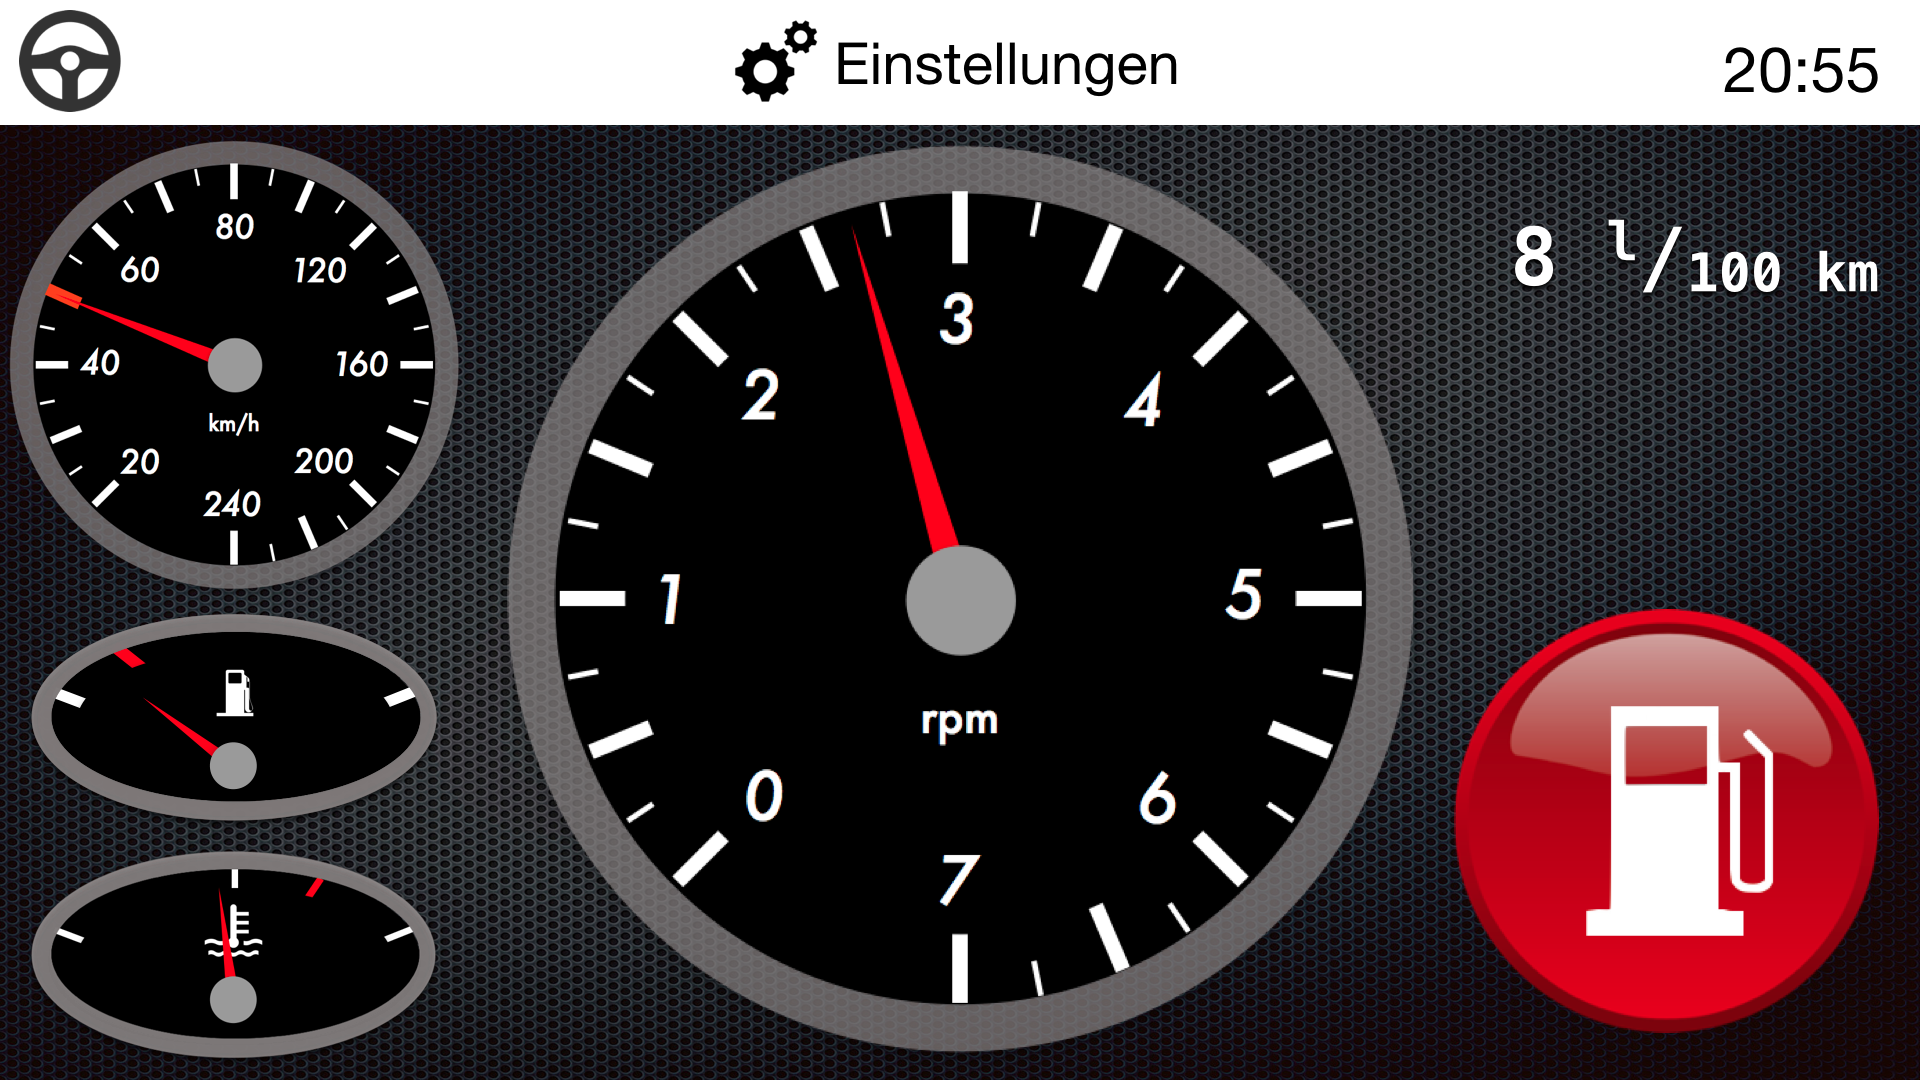
\includegraphics[width=\textwidth]{Images/GUI-Dashboard.png}
  		\caption{Verschiedene Dash-Anzeigeelemente.}
  	\end{center}
\end{figure}

\clearpage
\section{Grid}

Das Dashboard ist als Gitter(Grid) aufgebaut. Die Anzahl der Zeilen und Spalten hängen von der Bildschirmgröße des Endgeräts ab. Hier wird also z.B. auf einem Smartphone ein 8x4-Gitter angezeigt während auf einem Computerbildschirm z.B. ein 16x9-Gitter.

Welche Dashes im allgemeinen angezeigt werden, kann über die Einstellungsansicht konfiguriert werden. Wenn man in dieser weitere Anzeigeelemente hinzufügt werden diese in die noch verfügbaren Rechtecke platziert. Zur Not werden dann rechts noch weitere Rechtecke erzeugt die durch scrolling erreicht werden können.

Durch längeres Drücken und darauffolgendes Bewegen eines Elementes lässt es sich verschieben. Ohne das Bewegen werden zwei Schaltflächen angezeigt. Eine um das Dash zu entfernen, das andere um die Größe des Dashs zu verändern. Die Größe bleibt jedoch proportional und im Rahmen des Gitters. Hier werden dann z.B. aus 1x1-Anzeigen 2x2-Anzeigen, oder aus 1x2-Dashes 2x4-Anzeigen. In einem 8x4-Gitter sind jedoch keine 5x5-Anzeigen möglich.

Durch das verschieben werden andere Anzeigeelemente auch passend verschoben. Bei dem folgenden Bild z.B., wenn man das Dash in der Mitte nach links verschiebt werden die links platzierten Anzeigen automatisch nach rechts verschoben.

\begin{figure}[H]
  	\begin{center}
 		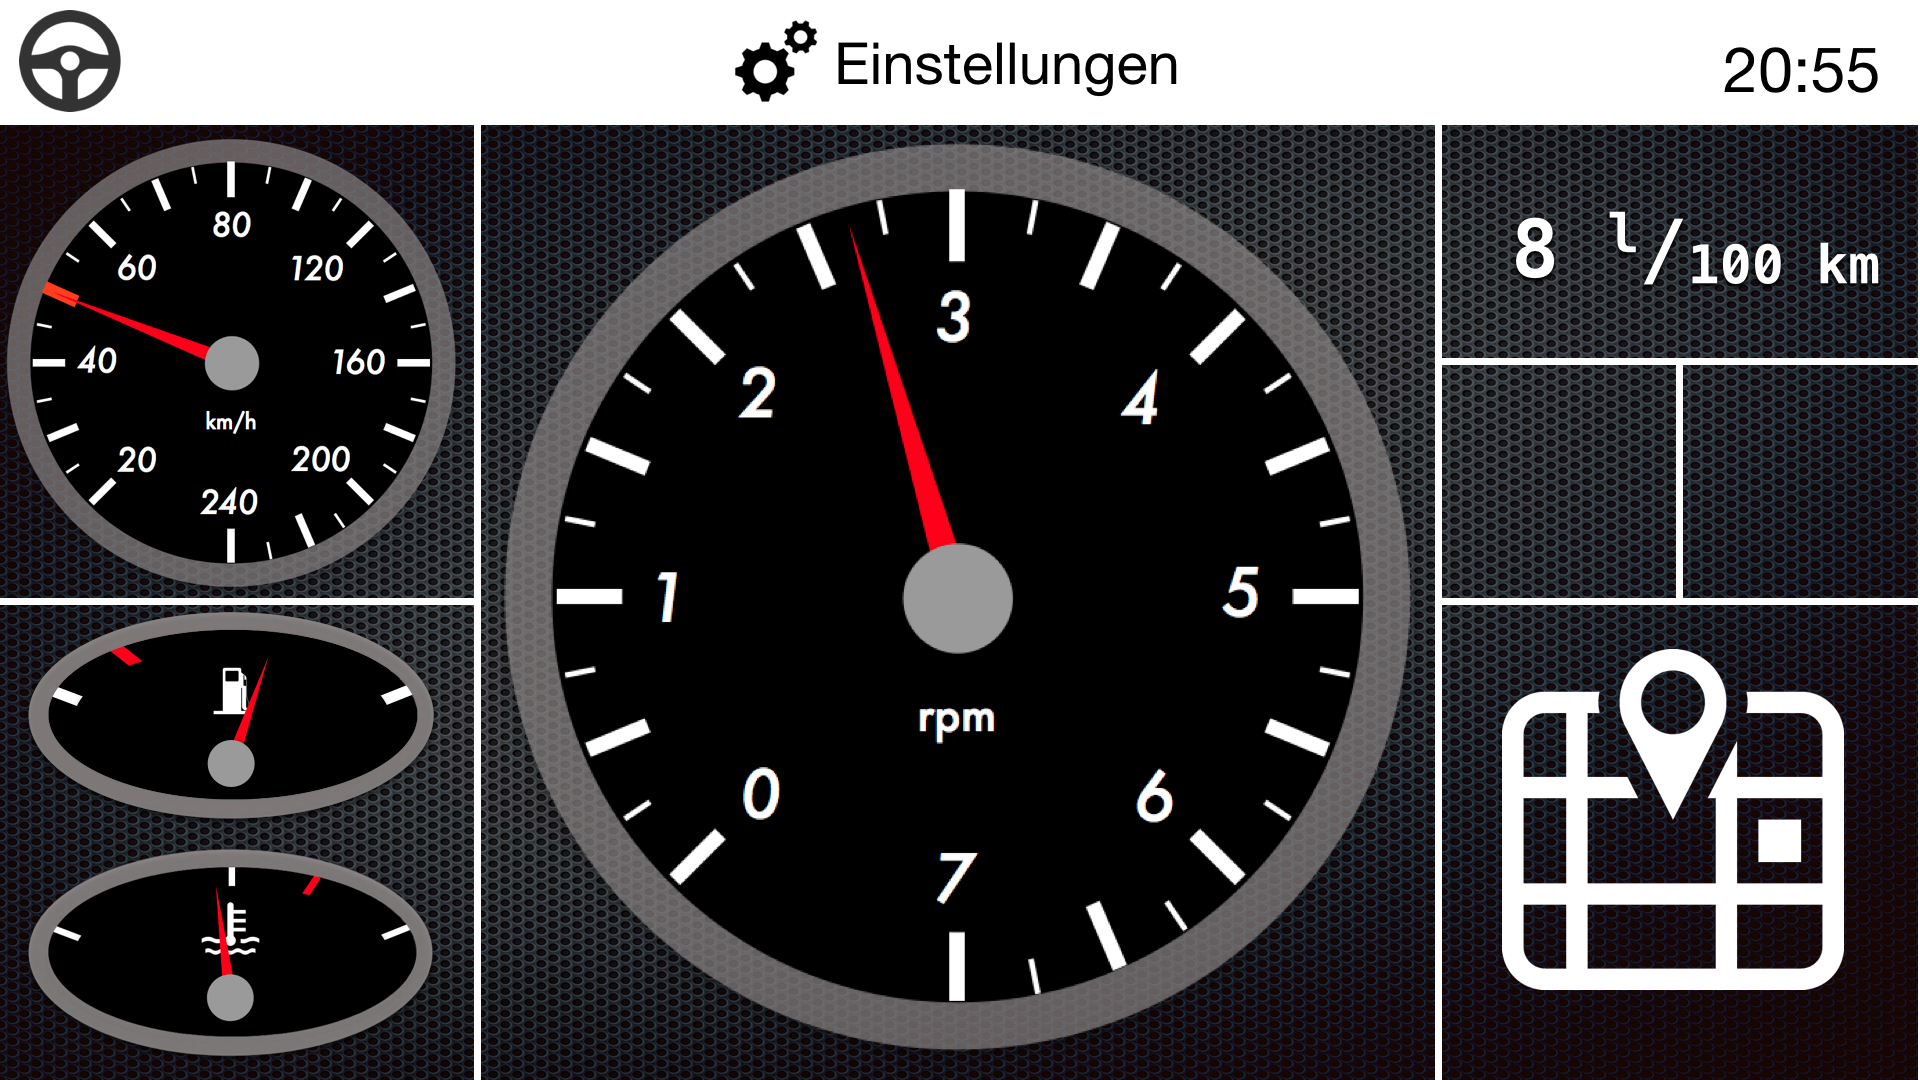
\includegraphics[width=\textwidth]{Images/GUI-DashboardGrid2.png}
  		\caption{Verschiedene Dash-Anzeigeelemente mit eingeblendeten Grid-Grenzen.}
  	\end{center}
\end{figure}

\clearpage
\section{Scrolling}

Wenn die Rechtecke im Anzeigefenster für die gewünschten Dashes nicht ausreichen ist es möglich die komplette Anzeige horizontal zu scrollen. Hier werden rechts neue Rechtecke hinzugefügt falls versucht wird ein Dash an den rechten Rand, nicht nur in die rechtsgelegenen Rechtecke, der Anzeige zu schieben. Beim scrollen bleibt das Dashboard so stehen, dass keine abgeschnittenen Rechtecke angezeigt werden. 

\begin{figure}[H]
  	\begin{center}
 		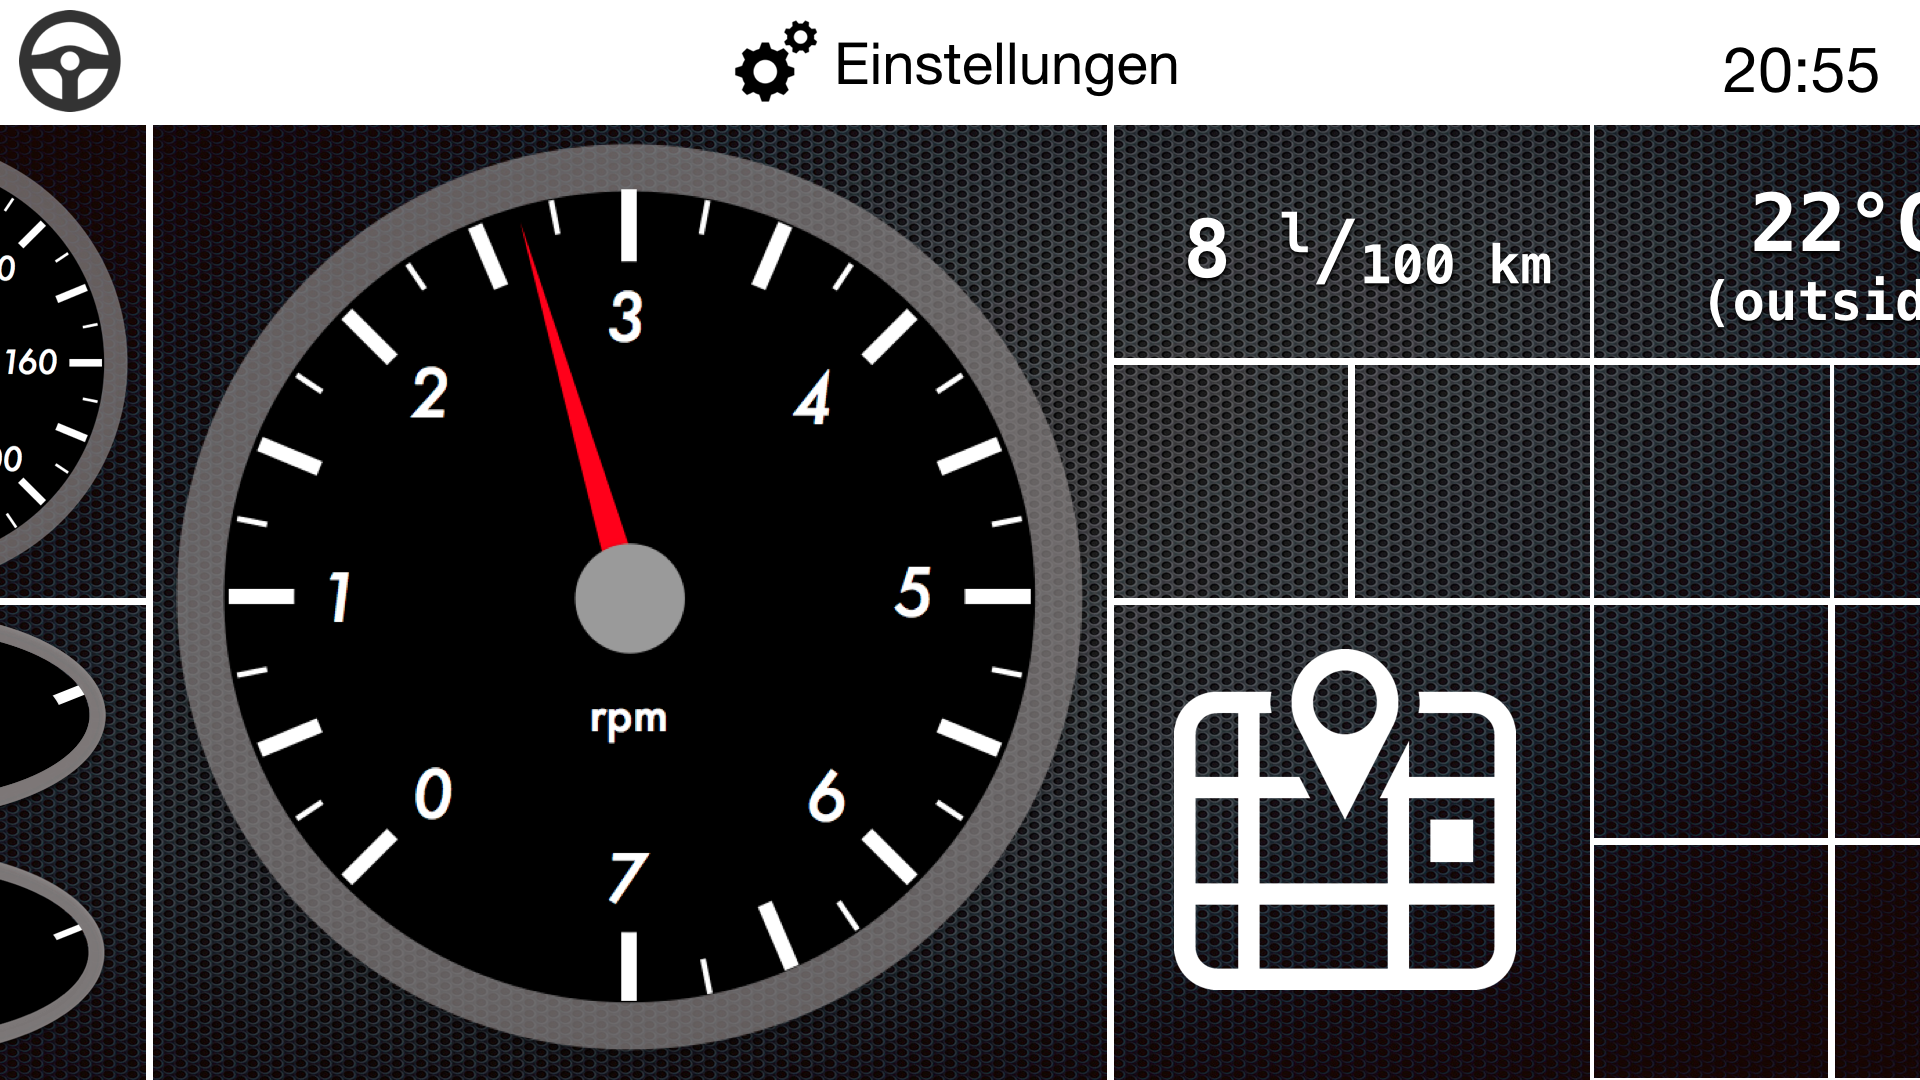
\includegraphics[width=\textwidth]{Images/GUI-DashboardGridScrolling.png}
  		\caption{Ein Dashboard während dem Scrollen.}
  	\end{center}
\end{figure}

\clearpage
\section{Größen}

Wie bereits weiter oben beschrieben gibt es verschiedene Anzeigeelemente die auch in verschiedenen Größen konfiguriert werden können. Hier ein Beispiel in dem in der Mitte eine einfache Geschwindigkeitsanzeige als 4x4-Element angezeigt wird. 
Es gibt jedoch nicht nur quadratische Elemente, wie man links unten sehen kann. Hier gibt es z.B. eine 2x1-Anzeige des Tankfüllstands und der Wassertemperatur. 
Außerdem gibt es neben runden und visuelle Anzeigen auch textuelle Dashes wie z.B. in der oberen rechten Ecke.

\begin{figure}[H]
  	\begin{center}
 		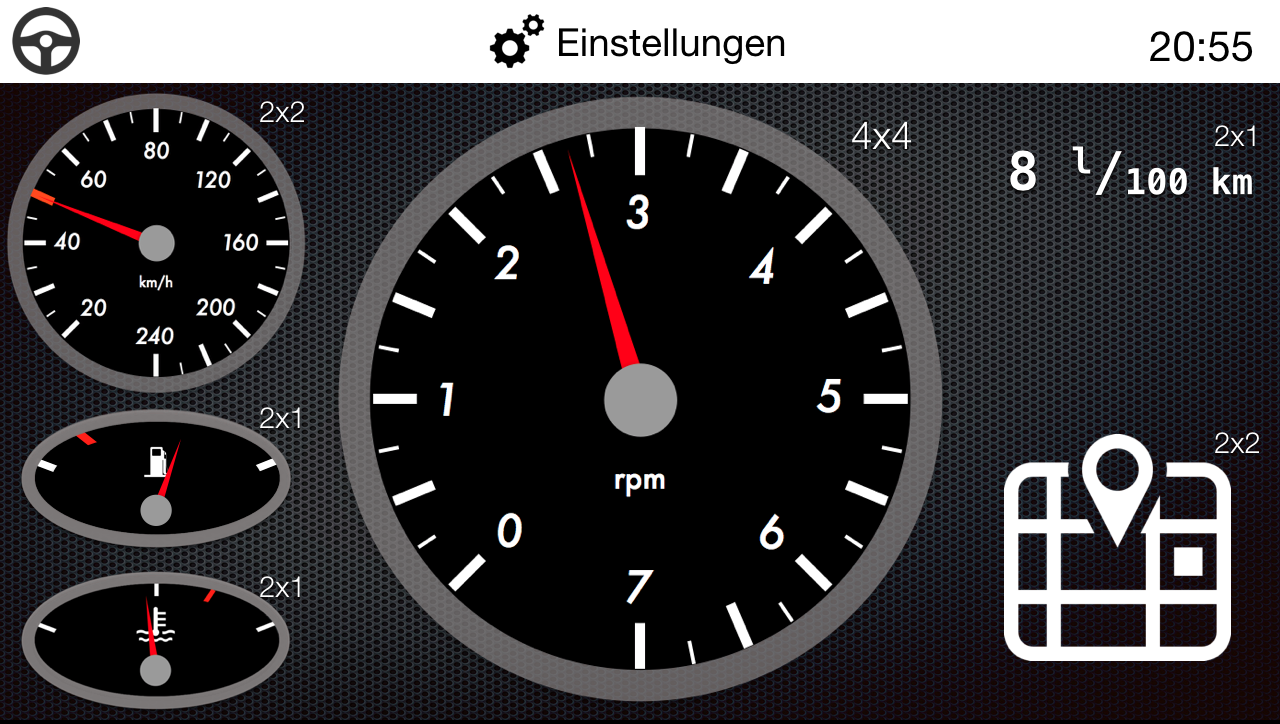
\includegraphics[width=\textwidth]{Images/GUI-DashboardSize.png}
  		\caption{Verschiedene Dash-Anzeigeelemente mit Grid-Größen}
  	\end{center}
\end{figure}

\clearpage
\section{Dashboard mit Statistik}

Weitere mögliche Anzeigeelemente neben Live-Anzeigen sind Graphen, auf denen Statistiken eines Wertes angezeigt werden können. In diesem Beispiel kann man z.B. die Geschwindigkeit über einen bestimmten Zeitraum, sowie den Kraftstoffverbrauch in zwei Graphen sehen. Zusätzlich sind noch weitere visuelle Anzeigen sichtbar.
\begin{figure}[H]
  	\begin{center}
 		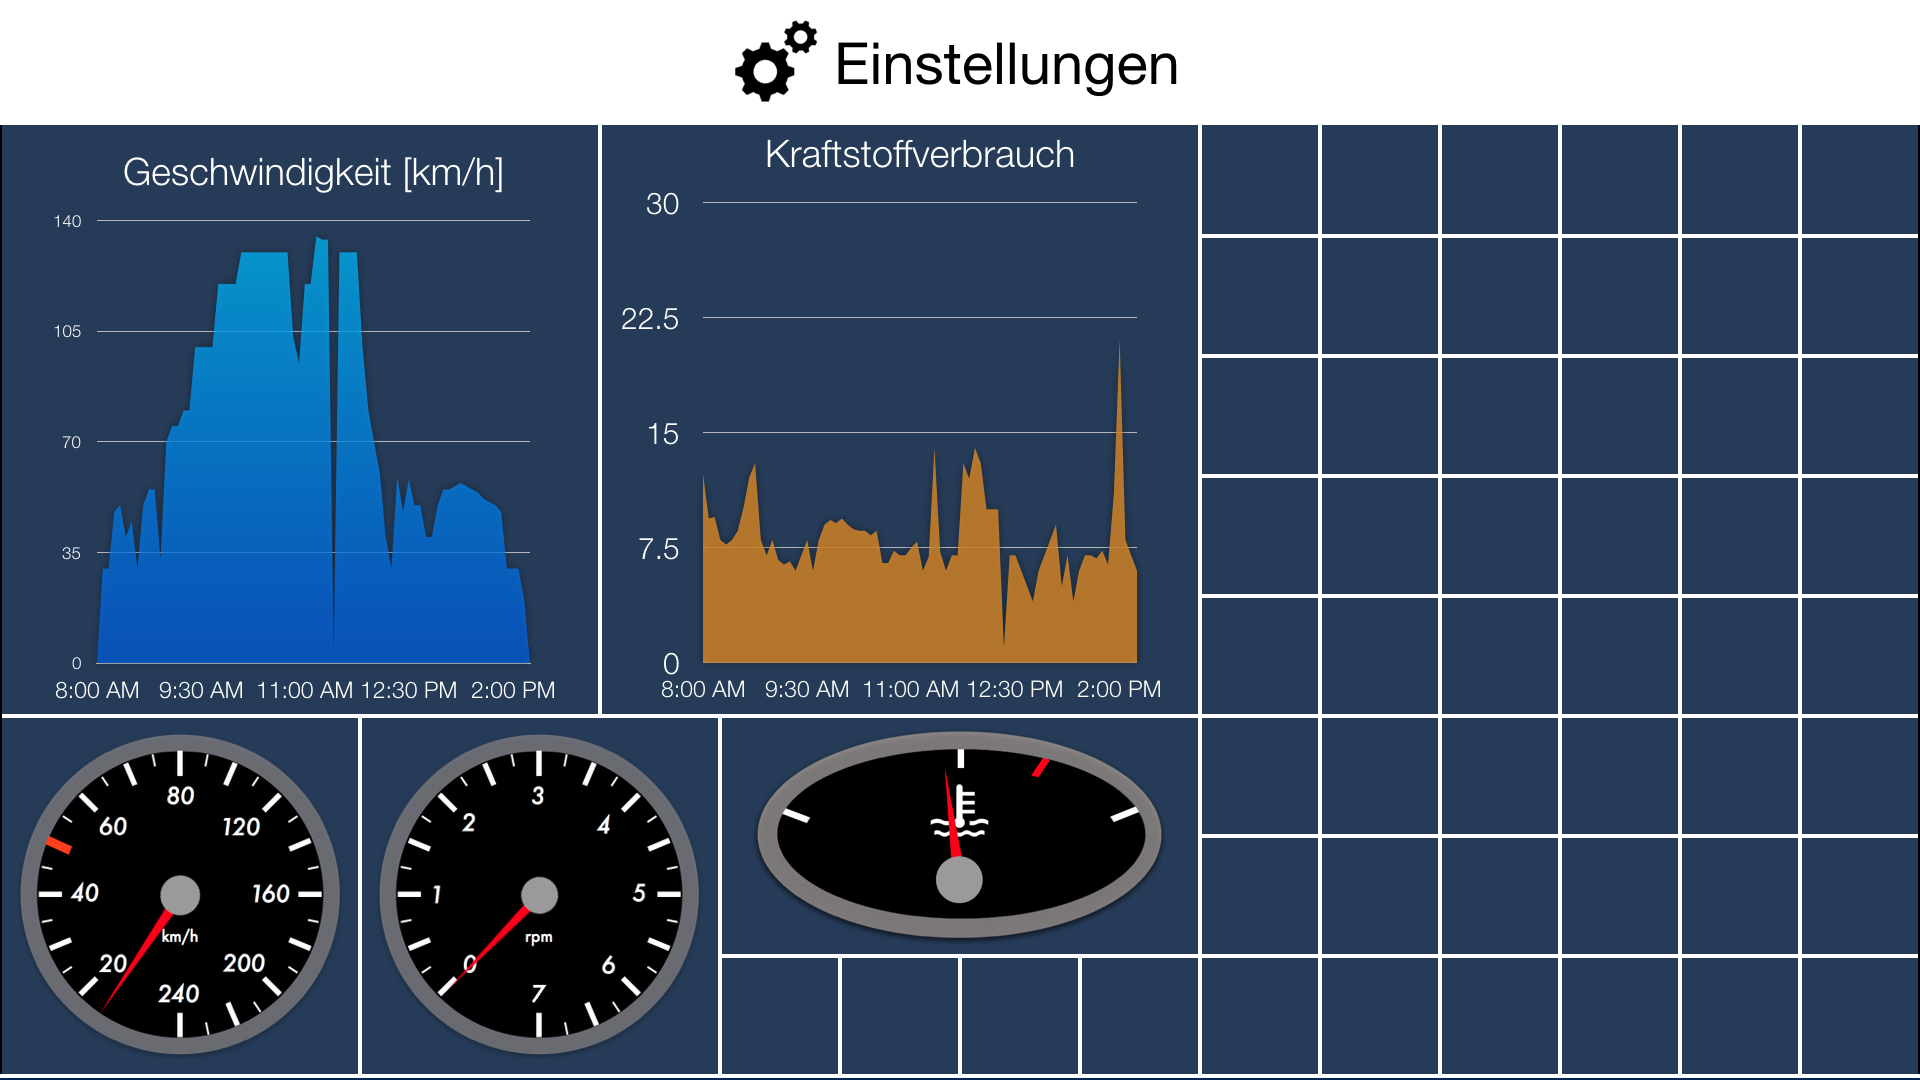
\includegraphics[width=\textwidth]{Images/GUI-DashboardStatistic.png}
  		\caption{Statistiken mit anderen Anzeigeelementen.}
  	\end{center}
\end{figure}

\clearpage
\section{Tabellen}

Die Tabelle kann in verschiedenen Anzeigen genutzt werden. Die Tabellengröße, also die Anzahl der Spalten und Zeilen, ist variabel. In der Tabelle kann man scrollen und ihre Zellen können mit verschiedenen Elementen, wie z.B. Bildern oder Text, gefüllt werden. Bei Berührung einer Zelle kann eine Funktion aufgerufen werden.\\
Genutzt wird eine Tabelle z.B. in der ~\nameref{sec:Karte}. 

\begin{figure}[H]
  	\begin{center}
 		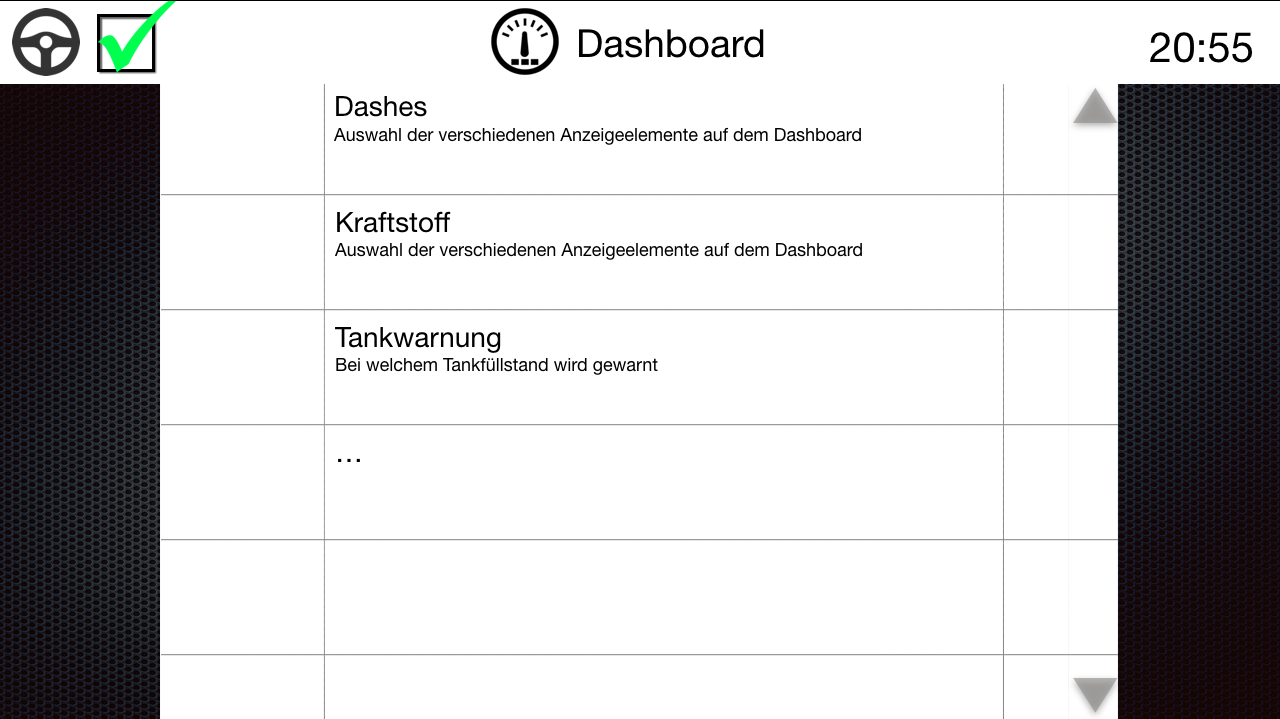
\includegraphics[width=\textwidth]{Images/GUI-Settings.png}
  		\caption{Beispiel: Tabelle mit den verschiedenen verfügbaren Informationen.}
  	\end{center}
\end{figure}


Eine Anzeige, in der die Tabelle sogar hauptsächlich zur Anwendung kommt, sind Einstellungen. 


\clearpage
\section{Einstellungen}
Hier werden zuerst alle Einstellungskategorien in der Tabelle angezeigt, diese sind die Anzeigeelemente und Allgemeine Konfigurationen wie der "niedrige Tankfüllstand". Bei Druck auf eine Kategorie wird die Anzeige der gewählten Kategorie geöffnet. Hier werden in einer Tabelle die verschiedenen Konfigurationsmöglichkeiten dargestellt. Diese lassen sich auch wieder über einen Druck auf das Tabellenelement beeinflussen. 
%Hier wird dann eine kleine Tabelle mit den Optionen oder falls nötig ein beschreibbares Textfeld angezeigt.
In dem folgenden Beispiel wird die Auswahl der Dashes angezeigt. Hier lässt sich ein Element per Druck auswählen und wieder abwählen. Der Status wird über den Haken angezeigt.

In den gesamten Einstellungen kann man sich oben rechts über das Kästchen mit dem Haken zum Fahrer machen.

Das verlassen der Tabelle ist möglich über die mittig in der obigen Leiste befindliche Schaltfläche mit dem Namen der letzten Anzeige. Hier ist es z.B. möglich aus der obersten Einstellungsanzeige wieder auf das Dashboard zu wechseln. Vorgenommene Einstellungen werden erst bei verlassen der Einstellungen aktiv.  


\clearpage
\section{Karte}
\label{sec:Karte}

Eine weitere Ansicht ist die Karte. Hier wird links eine Tabelle genutzt, um z.B. Werkstätten oder Tankstellen in der Nähe vorzuschlagen. Rechts werden diese dann in einer Karte zusammen mit dem aktuellen Standort angezeigt.
Bei Auswahl einer der Vorschläge wird auf der Karte die relative Position zum Auto angezeigt.
\begin{figure}[H]
  	\begin{center}
 		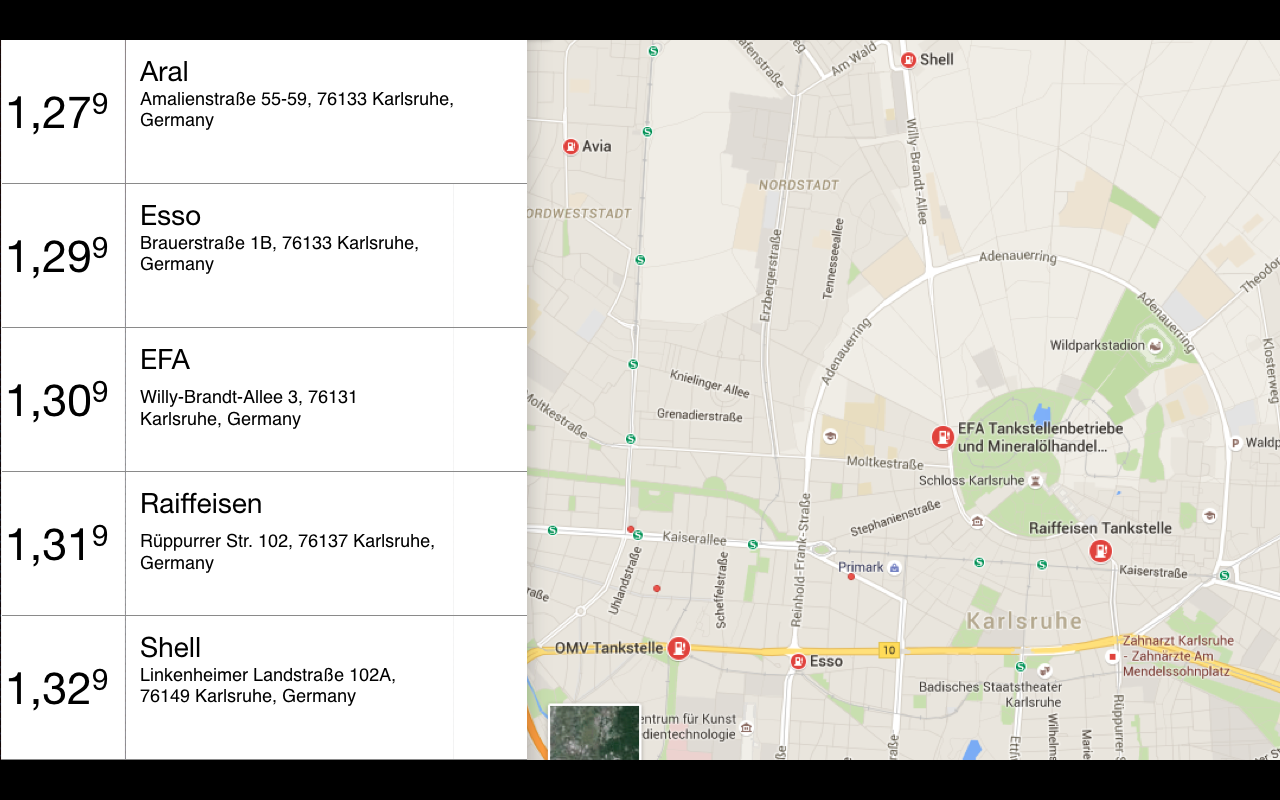
\includegraphics[width=\textwidth]{Images/GUI-Map.png}
  		\caption{Eine Kartenanzeige mit einer Tabelle}
  	\end{center}
\end{figure}

\clearpage
\section{Rückfahrkamera}

Die Rückfahr-Ansicht zeigt dem Nutzer, falls verfügbar, die aktuelle Fahrbahn über eine Kurve auf dem Kamerabild sowie, die Ultraschalldaten visualisiert über das Ampelsystem an der passenden unteren Seite des Kamerabildes. Erreichbar ist diese Ansicht durch eine Schaltfläche ähnlich dem Karten-Button.

\begin{figure}[H]
  	\begin{center}
 		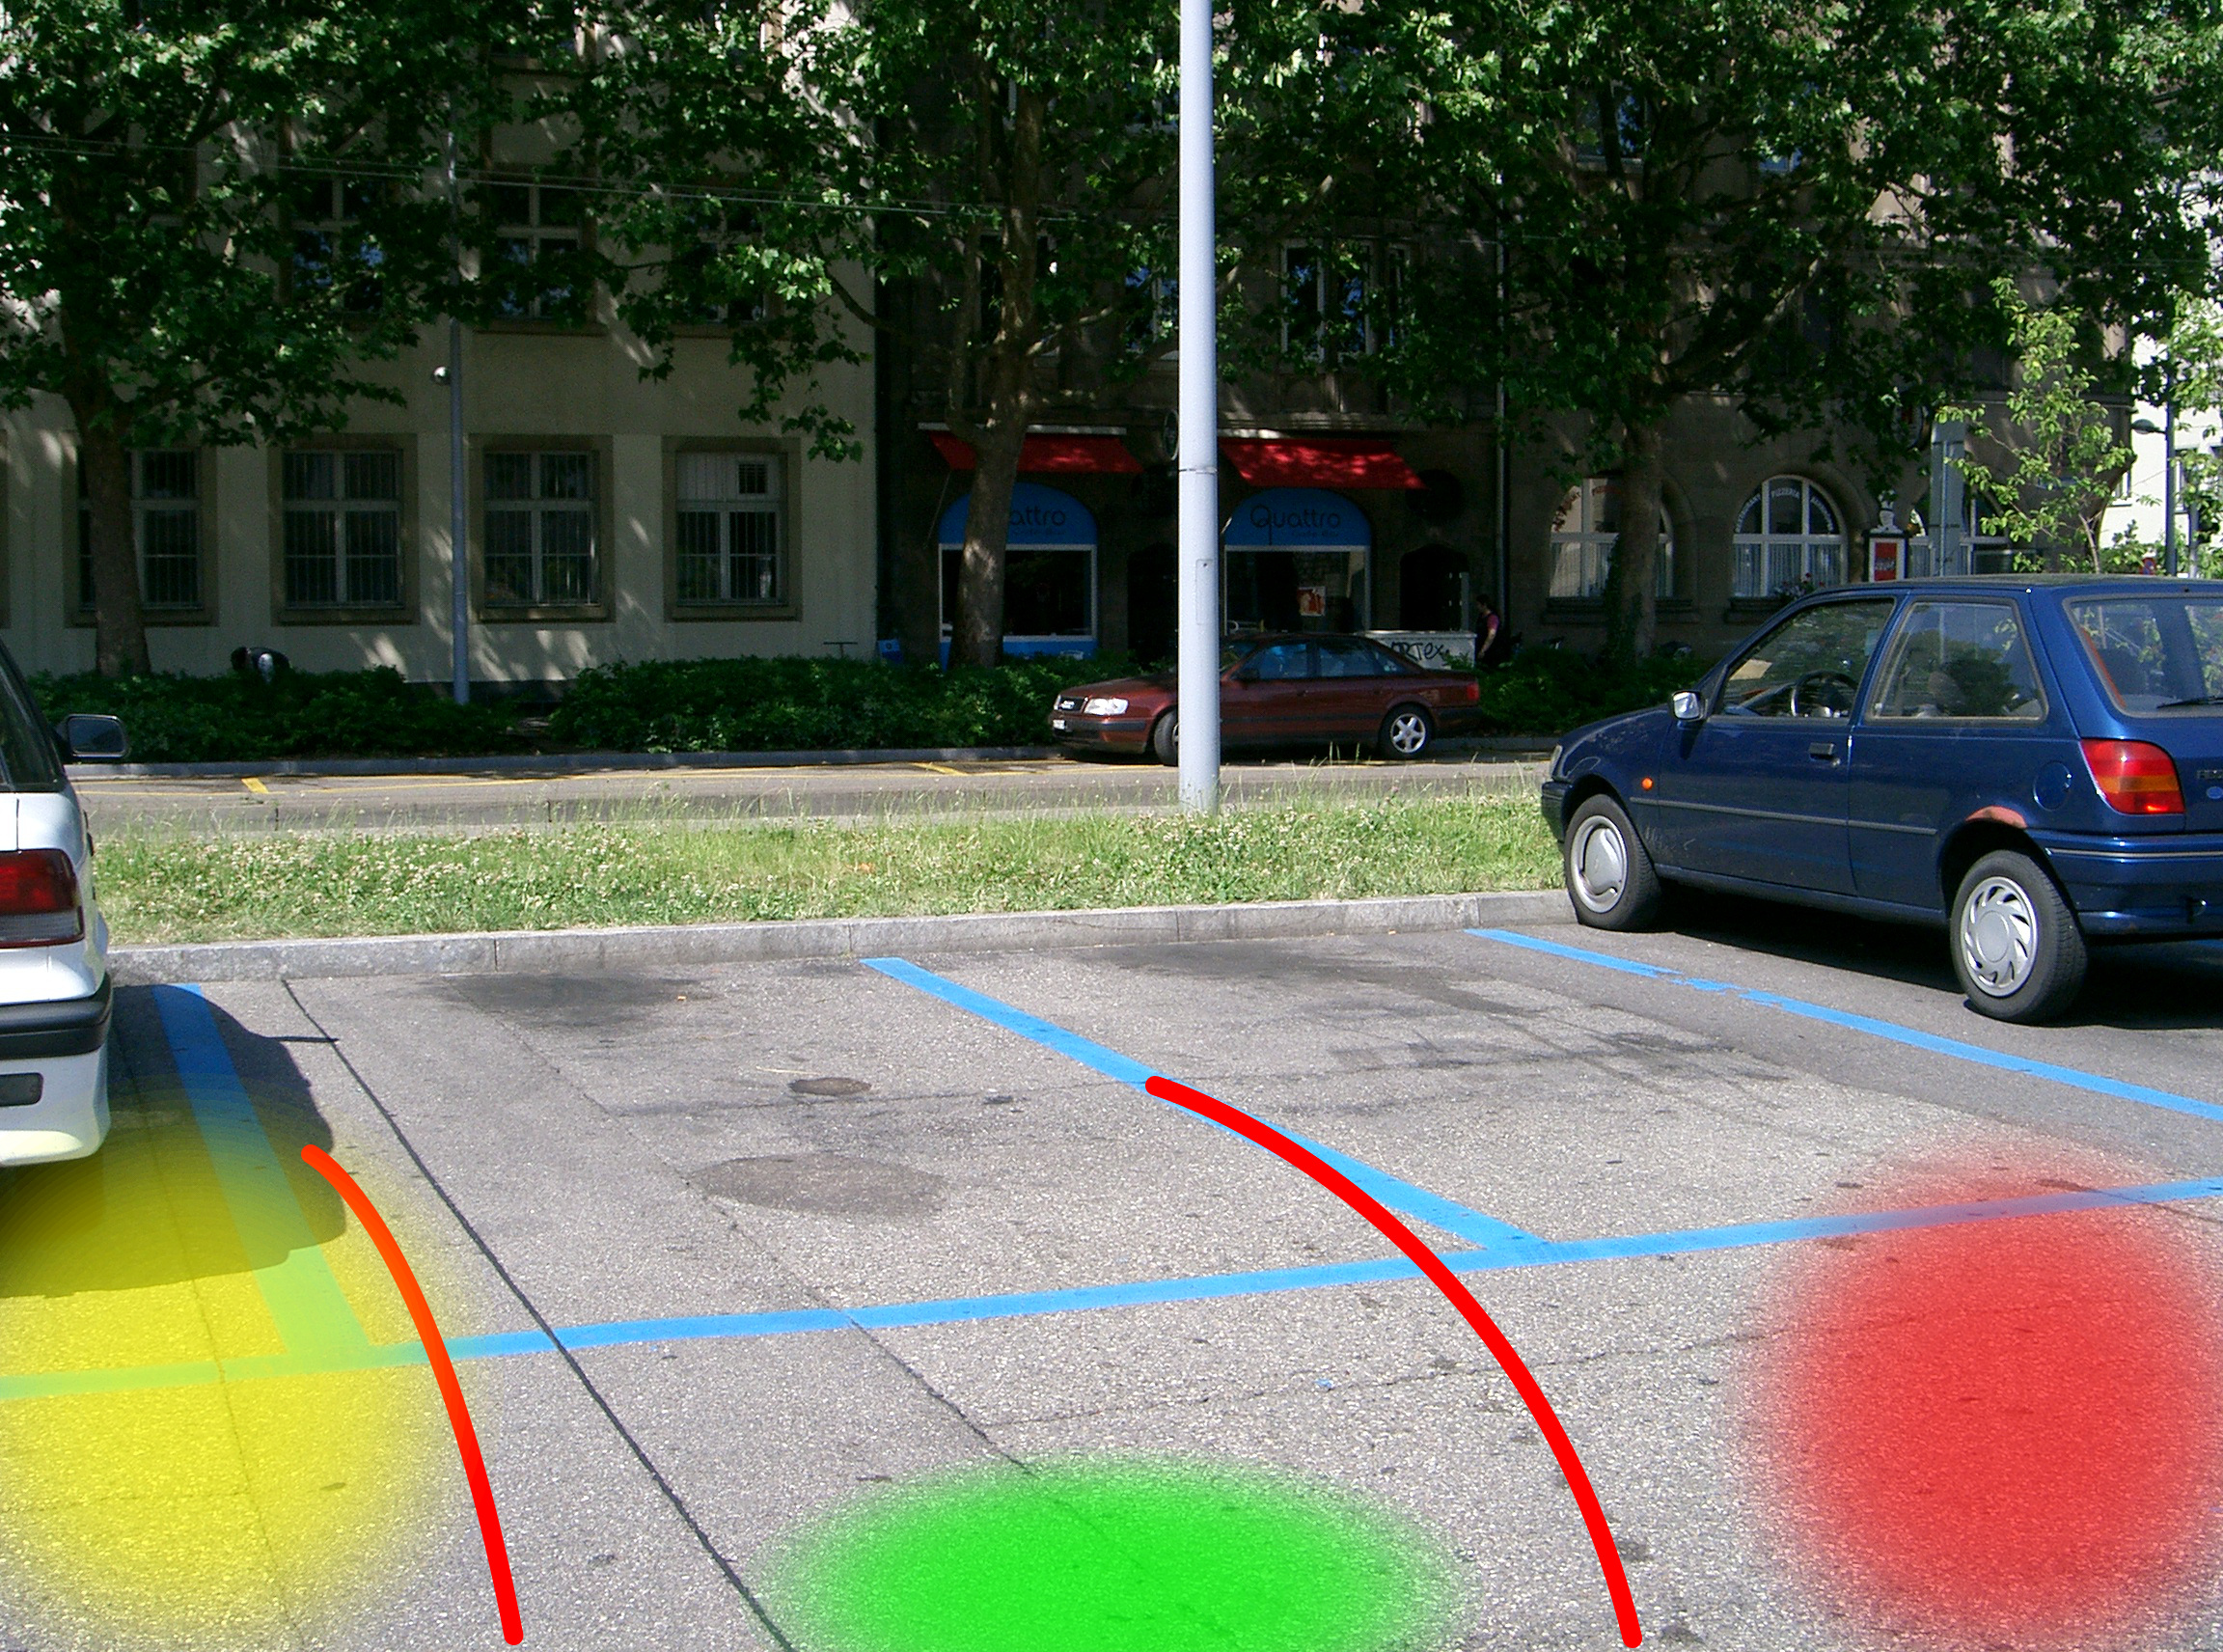
\includegraphics[width=\textwidth]{Images/GUI-BackDrive.jpg}
  		\caption{Kamerabild mit eingeblendeter Fahrbahn und Abstandswerten.}
  	\end{center}
\end{figure}

\end{document}